\documentclass[sigplan, review]{acmart}

\usepackage{booktabs} % For formal tables

% To include figures
\usepackage{graphicx}

% For TiKZ plots
\usepackage{tikz,pgfplots}

% To typeset SYCL programs
\usepackage{sycl}

% URL looks nicer in Teletype style
\urlstyle{tt}

% Copyright
%\setcopyright{none}
%\setcopyright{acmcopyright}
%\setcopyright{acmlicensed}
\setcopyright{rightsretained}
%\setcopyright{usgov}
%\setcopyright{usgovmixed}
%\setcopyright{cagov}
%\setcopyright{cagovmixed}


% DOI
%\acmDOI{10.475/123_4}

% ISBN
%\acmISBN{123-4567-24-567/08/06}

%Conference
\acmConference[DHPCC'2017]{Distributed \& Heterogeneous Programming in
  C/C++ Workshop 2017}{May 2017}{Toronto, Canada}

\acmMonth{5}
\acmYear{2017}

%\acmPrice{15.00}

%\acmBadgeL[http://ctuning.org/ae/ppopp2016.html]{ae-logo}
%\acmBadgeR[http://ctuning.org/ae/ppopp2016.html]{ae-logo}

\sloppy
\begin{document}

\title{SYCL C++17 and OpenCL interoperability experimentation with
  triSYCL}

\author{Anastasios Doumoulakis}
\email{anastasi@xilinx.com}

\author{Ronan Keryell}
\email{Ronan.Keryell@xilinx.com}

\author{Kenneth O'Brien}
\email{kennetho@xilinx.com}

\affiliation{%
  \institution{Xilinx Research Labs}
  \streetaddress{2020 Bianconi Avenue}
  \city{Dublin}
  \country{Ireland}
  \postcode{D24 T683}
}


\begin{abstract}
  Heterogeneous computing is required in systems ranging from low-end
  embedded systems up to the high-end HPC systems to reach
  high-performance while keeping power consumption low. Having more
  and more accelerators and CPU put also more challenges on the
  programmer, requiring even more expertise. Fortunately, new modern
  C++-based domain-specific languages such as SYCL allow to simplify
  the programming task at the full system level while keeping high
  performance.

  Besides its single-source programming aspect, the SYCL open standard
  from Khronos Group has an OpenCL interoperability mode, allowing to
  reuse existing OpenCL code inside the SYCL framework to simplify and
  optimize the data transfers between host and devices.

  We present some experiments on 2 applications on GPU and FPGA with
  the triSYCL open-source implementation.
\end{abstract}

%
% The code below should be generated by the tool at
% http://dl.acm.org/ccs.cfm
\begin{CCSXML}
<ccs2012>
<concept>
<concept_id>10010147.10010169.10010175</concept_id>
<concept_desc>Computing methodologies~Parallel programming languages</concept_desc>
<concept_significance>500</concept_significance>
</concept>
<concept>
<concept_id>10010147.10010169.10010170.10010174</concept_id>
<concept_desc>Computing methodologies~Massively parallel algorithms</concept_desc>
<concept_significance>300</concept_significance>
</concept>
<concept>
<concept_id>10011007.10011006.10011008.10011009.10010175</concept_id>
<concept_desc>Software and its engineering~Parallel programming languages</concept_desc>
<concept_significance>500</concept_significance>
</concept>
<concept>
<concept_id>10011007.10011006.10011050.10011017</concept_id>
<concept_desc>Software and its engineering~Domain specific languages</concept_desc>
<concept_significance>500</concept_significance>
</concept>
<concept>
<concept_id>10011007.10011006.10011066.10011067</concept_id>
<concept_desc>Software and its engineering~Object oriented frameworks</concept_desc>
<concept_significance>300</concept_significance>
</concept>
<concept>
<concept_id>10010520.10010521.10010542.10010546</concept_id>
<concept_desc>Computer systems organization~Heterogeneous (hybrid) systems</concept_desc>
<concept_significance>300</concept_significance>
</concept>
</ccs2012>
\end{CCSXML}

\ccsdesc[500]{Computing methodologies~Parallel programming languages}
\ccsdesc[300]{Computing methodologies~Massively parallel algorithms}
\ccsdesc[500]{Software and its engineering~Parallel programming languages}
\ccsdesc[500]{Software and its engineering~Domain specific languages}
\ccsdesc[300]{Software and its engineering~Object oriented frameworks}
\ccsdesc[300]{Computer systems organization~Heterogeneous (hybrid) systems}
% We no longer use \terms command
%\terms{Theory}

\keywords{C++17, SYCL, DSeL, OpenCL, FPGA, GPU, triSYCL}


\maketitle

\section{Introduction}
\label{sec:introduction}

Computing architectures nowadays are huge hybrid multi-processor
system-on-chips with different kind of processors, GPU, configurable
specific accelerators (video CODEC...), reconfigurable programmable
logic (FPGA), various hierarchies of memory and memory interfaces,
configurable IO and network support, security support, power control,
etc. High-performance applications may use a hierarchy of such system
up to fill up a full-scale data-center.

So the programmer is facing nowadays a fractal architecture, demanding
also more and more control for power efficiency. This tends to require
a dense fractal set of skills and tools.

SYCL \cite{SYCL-1.2} is a new open standard from Khronos
Group aiming at solving some of the programming issues related to
heterogeneous computing.  This pure C++17 domain-specific embedded
language allows the programmer to write single-source C++17 host code
with accelerated code expressed as functors. The data accesses are
described with accessor objects that implicitly define a task graph
that can be asynchronously scheduled on a distributed-memory system
including several CPU and accelerators.

This programming model is quite generic but provides also an
interoperability mode with the OpenCL realm, another standard from
Khronos Group aimed at heterogeneous computing with a C host API and
separate language for the kernels (C, C++, SPIR and SPIR-V).  This
allows a SYCL C++ application to recycle existing OpenCL kernels into
a higher level C++ programming model, relieving the programmer from
explicitly defining the memory transfers.

In this article we present in Section~\ref{sec:sycl} the SYCL
standard, then in Section~\ref{sec:sycl-opencl-inter} to finish in
Section~\ref{sec:exper-with-opencl} with some experiments with the
triSYCL open source implementation of the SYCL standard and comparing
to some related work in Section~\ref{sec:related-work}.


\section{SYCL}
\label{sec:sycl}

\begin{figure*}
  \begin{tabular}{c}
    \begin{lstlisting}[basicstyle=\scriptsize]
// Demonstrate the use of an asynchronous task graph of kernels to
// initialize and addition 2 matrices.
#include <CL/sycl.hpp>
#include <iostream>

using namespace cl::sycl;

// Size of the matrices
constexpr size_t N = 2000;
constexpr size_t M = 3000;

int main() {
  // Create a queue to work on
  queue q;

  // Create some 2D buffers of N*M floats for our matrices
  buffer<float, 2> a { { N, M } };
  buffer<float, 2> b { { N, M } };
  buffer<float, 2> c { { N, M } };

  // Launch a first asynchronous kernel to initialize a
  q.submit([&] (handler &cgh) {
      // The kernel write a, so get a write accessor on it
      auto A = a.get_access<access::mode::write>(cgh);

      // Enqueue a parallel kernel iterating on a N*M 2D iteration space
      cgh.parallel_for<class init_a>({ N, M },
                                     [=] (id<2> index) {
                                       A[index] = index[0]*2 + index[1];
                                     });
    });

  // Launch an asynchronous kernel to initialize b
  q.submit([&] (handler &cgh) {
      // The kernel write b, so get a write accessor on it
      auto B = b.get_access<access::mode::write>(cgh);
      /* From the access pattern above, the SYCL runtime detect this
         command group is independent from the first one and can be
         scheduled independently */

      // Enqueue a parallel kernel iterating on a N*M 2D iteration space
      cgh.parallel_for<class init_b>({ N, M },
                                     [=] (id<2> index) {
                                       B[index] = index[0]*2014 + index[1]*42;
                                     });
    });

  // Launch an asynchronous kernel to compute matrix addition c = a + b
    q.submit([&] (handler &cgh) {
        // In the kernel a and b are read, but c is written
        auto A = a.get_access<access::mode::read>(cgh);
        auto B = b.get_access<access::mode::read>(cgh);
        auto C = c.get_access<access::mode::write>(cgh);
        // From these accessors, the SYCL runtime will ensure that when
        // this kernel is run, the kernels computing a and b completed

        // Enqueue a parallel kernel iterating on a N*M 2D iteration space
        cgh.parallel_for<class matrix_add>({ N, M },
                                           [=] (id<2> index) {
                                             C[index] = A[index] + B[index];
                                           });
      });

    /* Request an access to read c from the host-side. The SYCL runtime
       ensures that c is ready when the accessor is returned */
    auto C = c.get_access<access::mode::read>();
    std::cout << std::endl << "Result:" << std::endl;
    for (size_t i = 0; i < N; i++)
      for (size_t j = 0; j < M; j++)
        // Compare the result to the analytic value
        if (C[i][j] != i*(2 + 2014) + j*(1 + 42)) {
          std::cout << "Wrong value " << C[i][j] << " on element "
                    << i << ' ' << j << std::endl;
          exit(-1);
        }

  std::cout << "Good computation!" << std::endl;
  return 0;
}
    \end{lstlisting}
  \end{tabular}
  \caption{Example of a SYCL C++ program producing and adding 2
    matrices, coming from from
    \url{https://github.com/triSYCL/triSYCL/blob/master/tests/examples/demo_parallel_matrix_add.cpp}.\label{fig:SYCL-example}}
\end{figure*}

SYCL \cite{SYCL-1.2,SYCL-2.2-provisional} (pronounced ``sickle'') is a
royalty-free, cross-platform abstraction C++ programming model for
OpenCL \cite{OpenCL-API-2.2-provisional,
  OpenCL-C++-2.2-provisional}. SYCL builds on the underlying concepts,
portability and efficiency of OpenCL while adding much of the ease of
use and flexibility of single-source C++.

Developers using SYCL are able to write standard C++14/C++17 code,
with many of the techniques they are accustomed to, such as
inheritance and templating. At the same time developers have access to
the full range of capabilities of OpenCL both through the features of
the SYCL libraries and, where necessary, through interoperation with
code written directly to the OpenCL
APIs~\cite{OpenCL-API-2.2-provisional}.

SYCL implements a single-source multiple compiler-passes design which
offers the power of source integration while allowing tool-chains to
remain flexible. This design supports embedding of code intended to be
compiled for an OpenCL device, for example a GPU or an FPGA, inline
with host code. This embedding of code offers three primary benefits:
\begin{description}
\item[simplicity:] for novice programmers, the separation of host and
  device source code in OpenCL can become complicated to deal with,
  particularly when similar kernel code is used for multiple different
  operations. A single compiler flow and integrated tool chain
  combined with libraries that perform a lot of simple tasks
  simplifies initial OpenCL programs to a minimum complexity. This
  reduces the learning curve for programmers new to OpenCL and allows
  them to concentrate on parallelization techniques rather than
  syntax;
\item[reuse:] C++'s type system allows for complex interactions
  between different code units and supports efficient abstract
  interface design and reuse of library code.  For example, a C++
  \lstinline{std::transform} or \lstinline{std::for_each} algorithm
  applied to an array of data may allow specialization on both the
  operation applied to each element of the array and on the type of
  the data;
\item[efficiency:] tight integration with the type system and reuse of
  library code enables a compiler to perform inlining of code and to
  produce efficient specialized device code based on decisions made in
  the host code without having to generate kernel source strings
  dynamically as done with other frameworks \cite{VexCL,
    Boost.Compute}.
\end{description}

SYCL is a pure single-source C++ DSeL (Domain-Specific Embedded
Language) providing simpler abstractions for heterogeneous
computing. On Figure~\ref{fig:SYCL-example} is presented a small
application using SYCL concepts to create a graph of 3 asynchronous
tasks to initialize 2 matrices and addition them before checking for
the final result.

The main interesting features that SYCL brings are:
\begin{description}

\item[asynchronous task graphs] to break an application in parallel
  pieces able to run on various accelerators or on the host, taking
  advantage of the CPU cores and accelerators of the platform;

\item[hierarchical parallelism] to take advantage inside a task of the
  common intrinsic parallelism found in accelerators as shown on
  Figure~\ref{fig:OpenCL-execution-model}, that can be expressed
  either as in OpenCL with ND-ranges (multi-dimensional iteration
  spaces) or in a similar hierarchical way on how it is done in OpenMP
  \cite{OpenMP-5.0-preview-1}, but with a nicer C++-friendly method
  based on lambda functions. The simpler hierarchical way relieves the
  programmer from using painful work-group synchronizations and is
  also more efficient on CPU and FPGA;

  \begin{figure}
    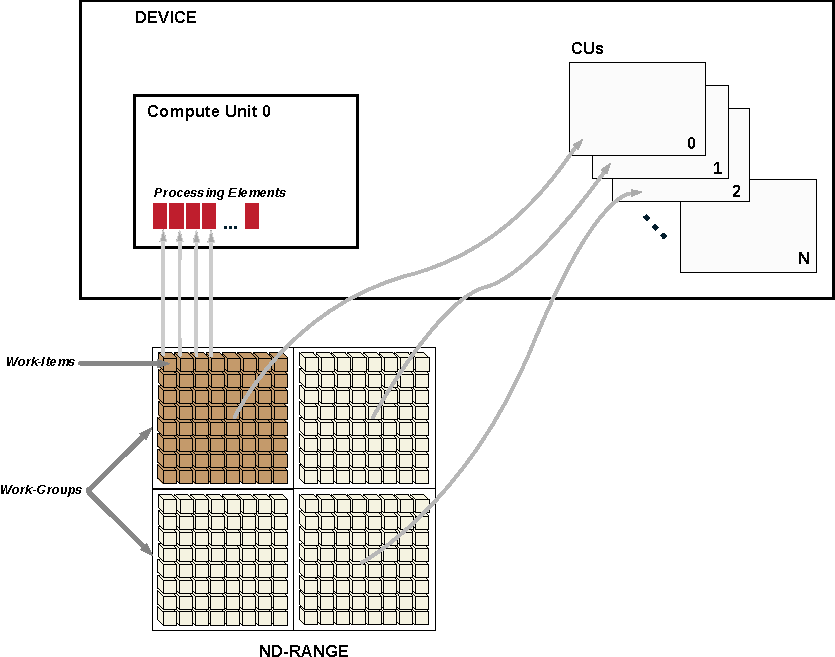
\includegraphics[width=\hsize]{figures/execution-model-no_GPU}
    \caption{OpenCL execution model, with the parallel iteration space
      of work-groups of work-items mapped for execution onto independent
    compute units composed of processing elements.}
    \label{fig:OpenCL-execution-model}
  \end{figure}

\item[buffers] defining location-independent storage (no explicit
  move) usable as multi-dimensional arrays to be used from the various
  CPU cores and accelerators;

\item[accessors] to express usage for buffers and other objects with
  some attributes such as read/write/\ldots, the location or the kind
  of memory to use, allowing finer control on the complex memory
  hierarchy found on accelerators as shown on
  Figure~\ref{fig:OpenCL-memory-model} to reach the maximum power and
  compute efficiency;

  \begin{figure}
    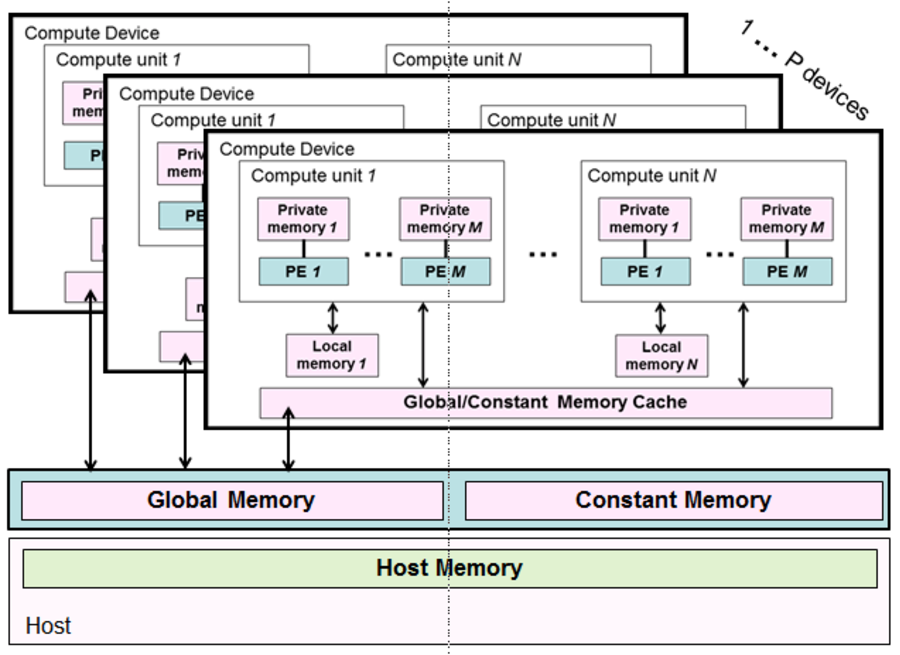
\includegraphics[width=\hsize]{figures/memory-model}
    \caption{OpenCL memory model, with the 4 different explicit kinds
      of memory, besides the host memory.}
    \label{fig:OpenCL-memory-model}
  \end{figure}

\item[implicit dependency graph] construction is done with the
  separation in SYCL of the data access from data storage. By relying
  on the C++-style RAII (resource acquisition is initialization) idiom
  on accessors, the runtime library can capture data dependencies
  between device code blocks and construct the task graph implicitly
  with all the dependencies;

\item[automatic data motion] is then done by the runtime by tracking
  the data through the accessors ahead of time, making sure the data
  are available when needed by a kernel on a device or by the host,
  without the programmer requiring like in OpenCL or in CUDA to
  explicitly move the data;

\item[overlapping kernels and communications] is provided
  automatically by the SYCL scheduler by using the dependency graph
  between tasks without requiring the programmer to manage explicitly
  several command queues and synchronizing events for this;

\item[single-source] programming model, taking advantage of OpenMP
  simplicity and type safety but in a pure C++-friendly world, without
  requiring \lstinline{#pragma} that do not compose nicely with
  C++. This allows the writing of high-level programming and
  meta-programming. For example on the Figure~\ref{fig:SYCL-example},
  except in the buffer creations on lines 17--19, the data type does
  not appear anywhere in the code and is just inferred by the compiler
  even across the host-device boundary;

\item[host fallback] is a by-product of having a pure C++ DSeL. By
  just providing a C++ implementation of the SYCL runtime on the
  host. Thus the same code can work either on the host CPU or on the
  device, allowing more parallelism but also just to run even if a
  device is missing;

\item[host debugging] for free is a nice side-effect of the host
  implementation of SYCL. The development of heterogeneous
  applications is quite challenging but having the same code running
  on the host allows the use of the normal C++ development tools
  chains, from high-end static analysis tools, dynamic thread or
  memory checkers, debuggers, watch-points, etc.  down to inserting
  plain standard I/O messages in the code;

\item[host emulation] is also for free, which interesting in the case
  of the FPGA world where really synthesizing the code for the device
  is very slow compared to running the code on CPU or even on GPU;

\item[cross-platform] support allows to have buffers used by different
  devices from different vendors in a seamless way, which is not
  possible directly in OpenCL.

  % Skip on purpose the OpenCL interoperability mode here

\end{description}

SYCL retains the execution model, runtime feature set and device
capabilities of the underlying OpenCL standard. This is why SYCL
1.2~\cite{SYCL-1.2} targets devices with OpenCL
1.2~\cite{OpenCL-API+C-1.2} capabilities, while SYCL
2.2~\cite{SYCL-2.2-provisional} targets devices with OpenCL
2.2~\cite{OpenCL-API-2.2-provisional} capabilities, adding for example
the pipes and the shared memory between the host and devices.

The OpenCL C specification imposes some limitations on the full range
of C++ features that SYCL is able to support. This ensures portability
of device code across as wide a range of devices as possible.

As a result, while the code can be written in standard C++ syntax with
interoperability with standard C++ programs, the entire set of C++
features is not available in SYCL device code. In particular, SYCL
device code, as defined by this specification, does not support
virtual function calls, function pointers in general, exceptions,
runtime type information or the full set of C++ libraries that may
depend on these features or on features of a particular host compiler.

Anyway these features are not often used in high-performance code even
in plain C++ in the hot-path because of performance issues.
Fortunately, the use of C++ features such as templates and inheritance
on top of the OpenCL execution model opens a wide scope for innovation
in software design for heterogeneous systems, giving workarounds for
some of the unsupported features.

Clean integration of device and host code within a single C++ type
system enables the development of modern, templated libraries that
build simple, yet efficient, interfaces to offer more developers
access to OpenCL capabilities and devices. SYCL is intended to serve
as a foundation for innovation in programming models for heterogeneous
systems, that builds on an open and widely implemented standard
foundation in the form of OpenCL.

This is why the OpenCL version of TensorFlow \cite{TensorFlow-1.0},
the C++ machine learning framework from Google, is actually using SYCL
instead of plain OpenCL.

SYCL is one of the candidates giving inputs on parallelism and
heterogeneous computing to the C++ ISO/IEC JTC1/SC22/WG21
standardization committee
\cite{C++:P00236R0:SYCL,C++:P0362R0,C++:P0363R0,C++:P0367R0}.
\iffalse
  WG21,
presented at C++ F2F committee Jacksonville 2016/02
% http://www.open-std.org/jtc1/sc22/wg21/docs/papers/2016/p0236r0.pdf
% https://groups.google.com/a/isocpp.org/forum/#!topic/sg14/8GWWDulGE7o
 Oulu 2016/06
% http://www.open-std.org/jtc1/sc22/wg21/docs/papers/2016/p0362r0.pdf
% http://www.open-std.org/jtc1/sc22/wg21/docs/papers/2016/p0363r0.pdf
% http://www.open-std.org/jtc1/sc22/wg21/docs/papers/2016/p0367r0.pdf
 Khronos committed to provide Open Source implementations of OpenCL and SYCL
\fi


\section{SYCL and OpenCL interoperability mode}
\label{sec:sycl-opencl-inter}

SYCL is a very generic data-parallel task graph model implemented as a
C++ DSeL that often relies on OpenCL and SPIR behind the hood to
target accelerators, but it could use some other technology.

There is also in SYCL a specific OpenCL interoperability mode if
needed, allowing direct interaction with the OpenCL world, and by
transitivity to Vulkan/OpenGL/DirectX/... In this way it is possible
to use existing programs or libraries with no overhead.

There are 2 main parts in the interoperability mode:
\begin{enumerate}
\item it is possible to construct SYCL objects from existing OpenCL
  objects to run SYCL single-source programs in relation with an
  existing OpenCL framework. For example a SYCL buffer can be
  constructed from an OpenCL \lstinline|cl_mem| or SYCL queue from a
  \lstinline|cl_command_queue|;
\item it is possible to extract OpenCL objects from higher-level SYCL
  objects to execute OpenCL code from the SYCL world, for example
  extract a \lstinline|cl_mem| from a SYCL accessor to launch an
  OpenCL kernel.
\end{enumerate}

Whereas the interoperability mode was included in the SYCL standard to
extend the applicability of SYCL on the OpenCL realm, it appears that
this mode is useful by itself to do plain OpenCL programming in higher
level C++, in the same way there exist already various C++ OpenCL
wrapper.

While it does not take advantage from the single-source programming
style of SYCL, it has some value for OpenCL programmers as it
simplifies the boilerplate and housekeeping. For example, it allows to
use the task graph model on top of OpenCL kernels and the synergy
between buffers and accessors relieves the programmer from managing
explicitly the buffer content transfers between host and devices.

In the following we present some use case of OpenCL interoperability
using the triSYCL implementation.


\section{Experimenting OpenCL interoperability mode of SYCL with
  triSYCL}
\label{sec:exper-with-opencl}

triSYCL \cite{triSYCL} is an open-source implementation based on C++17
and various Boost libraries \cite{Boost-1.63}. The device compiler used to
outline the kernels in single-source mode is based on Clang
\cite{Clang-4.0}/LLVM \cite{LLVM-4.0}. The OpenCL interoperability mode is
based on Boost.Compute \cite{Boost.Compute}.

Actually to even simplify further the programming style, triSYCL
implements Boost.Compute interoperability mode too, as an extension to
the SYCL standard.

We have used triSYCL to simplify the OpenCL host-side programming of
two applications related to machine learning.


\subsection{Handwritten digit recognition in gray images using L2
  norm}
\label{sec:example-from-anast}

To benchmark various languages and frameworks, we used an application
for recognition of handwritten digits in 8-bit gray images of
$28 \times 28$ pixels.

Basically there are 500 images compared against a training reference
set of labeled digit images. A kernel is launches to compare each
image against all the reference images.

\begin{figure}
  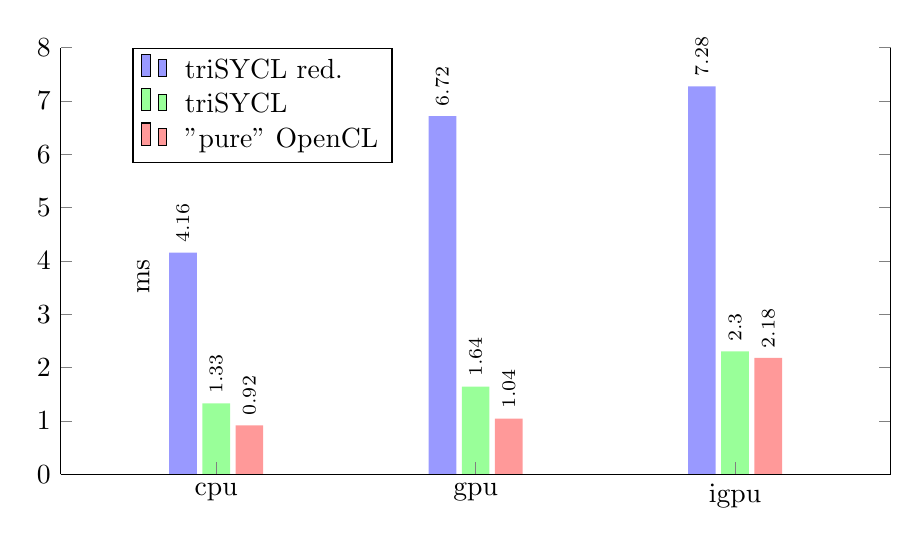
\begin{tikzpicture}
    \begin{axis}[ 
      ybar,
      axis on top,
      ymax=8, ymin=0, 
      height=7cm,
      width=\hsize, 
      enlarge x limits=0.3, 
      ymajorgrids, 
      tick align=inside,
      major grid style={draw=none}, 
      axis x line*=left,
      ylabel={ms}, 
      xtick=data, 
      legend cell align=left, 
      max space between ticks=20pt, 
      legend style={ at={(0.4,1.0)}, column sep=1ex },
      y label style={ at={(axis description cs:0.1,0.4)}, anchor=west},
      symbolic x coords={cpu, gpu, igpu}, 
      nodes near coords=\rotatebox{90}{\scriptsize\pgfmathprintnumber\pgfplotspointmeta},
      ]
      \addplot[draw=none,fill=blue!40!white] coordinates {(cpu, 4.158)
        (igpu, 7.275) (gpu, 6.717) };
      \addplot[draw=none,fill=green!40!white] coordinates {(cpu,
        1.329) (igpu, 2.303) (gpu, 1.642) };
      \addplot[draw=none,fill=red!40!white] coordinates {(cpu, 0.917)
        (igpu, 2.183) (gpu, 1.042) };

      \legend{triSYCL red., triSYCL, "pure" OpenCL}
    \end{axis}
  \end{tikzpicture}
  \caption{Average total execution time for digit recognition
    application per image.}
  \label{fig:results-digit-recognition}
\end{figure}

The examples with a SYCL, SYCL with OpenCL interoperability running
OpenCL kernel and a pure OpenCL implementations with the data sets can
be found on \url{https://github.com/a-doumoulakis/triSYCL_knn} for
further inspection.

\begin{figure*}
  \begin{tabular}{c}
    \begin{lstlisting}[basicstyle=\scriptsize]
  [...]

int search_image(buffer<int>& training, const Img& img, queue& q, const kernel& k) {
  int res[training_set_size];

  {
    buffer<int> A { std::begin(img.pixels), std::end(img.pixels) };
    buffer<int> B { res, training_set_size };
    // Compute the L2 distance between an image and each one from the
    // training set
    q.submit([&] (handler &cgh) {
        // Set the kernel arguments. The accessors lazily trigger data
        // transfers between host and device only if necessary. For
        // example "training" is only transfered the first time the
        // kernel is executed.
        cgh.set_args(training.get_access<access::mode::read>(cgh),
                     A.get_access<access::mode::read>(cgh),
                     B.get_access<access::mode::write>(cgh),
                     int { training_set_size }, int { pixel_number });
        // Launch the kernel with training_set_size work-items
        cgh.parallel_for(training_set_size, k);
      });
    // The destruction of B here waits for kernel execution and copy
    // back the data to res
  }

  // Find the image with the minimum distance
  auto min_image = std::min_element(std::begin(res), std::end(res));

  // Test if we found the good digit
  return
    training_set[std::distance(std::begin(res), min_image)].label == img.label;
}

int main(int argc, char* argv[]) {
  int correct = 0;
  training_set = slurp_file("data/trainingsample.csv");
  validation_set =  slurp_file("data/validationsample.csv");
  buffer<int> training_buffer = get_buffer(training_set);

  // A SYCL queue to send the heterogeneous work-load to
  queue q { boost::compute::system::default_queue() };

  // Use real OpenCL program for the kernel
  auto program = boost::compute::program::create_with_source(R"(
    __kernel void kernel_compute(__global const int* trainingSet,
                                 __global const int* data,
                                 __global int* res, int setSize, int dataSize) {
      int diff, toAdd, computeId;
      computeId = get_global_id(0);
      if (computeId < setSize) {
        diff = 0;
        for (int i = 0; i < dataSize; i++) {
            toAdd = data[i] - trainingSet[computeId*dataSize + i];
            diff += toAdd * toAdd;
        }
        res[computeId] = diff;
      }
    }
    )", boost::compute::system::default_context());

  program.build();

  // Construct a SYCL kernel from OpenCL kernel to be used in
  // interoperability mode
  kernel k { boost::compute::kernel { program, "kernel_compute"} };

  // Match each image from the validation set against the images from
  // the training set
  for (auto const & img : validation_set)
    correct += search_image(training_buffer, img, q, k);

  [...]

  return 0;
}
    \end{lstlisting}
  \end{tabular}
  \caption{Digit recognition application using SYCL with OpenCL
    interoperability mode.\label{fig:digit-SYCL-OpenCL-code}}
\end{figure*}


The main part of the SYCL with OpenCL interoperability version is
shown on Figure~\ref{fig:digit-SYCL-OpenCL-code}. Even the kernel is
described as OpenCL code with the help Boost.Compute
\cite{Boost.Compute} for conciseness, the data are still stored in
SYCL buffers and their usages are precised by some SYCL
accessors. Compared to the pure SYCL version found in
\url{https://github.com/a-doumoulakis/triSYCL_knn/blob/master/knn_trisycl.cpp},
we built a SYCL kernel from the OpenCL kernel and inside
\lstinline|q.submit()| the \lstinline|cgh.set_args()| connects the
SYCL world to the OpenCL kernel world, connecting the SYCL accessors
to some OpenCL \lstinline|cl_mem| provided to the OpenCL kernel during
execution. The OpenCL kernel is still scheduled asynchronously by the
SYCL runtime according to the task graph as would be a normal SYCL
kernel.

Even if there is no explicit OpenCL buffer motion between host and
device, the SYCL run-time uses the dependency graph constructed by the
accessors to move or not to move the data for kernel execution.

The performance results comparing a dumb triSYCL version with
redundant transfers between host and device as a
reference\footnote{The task graph is not used to optimize transfers or
  to limit OpenCL buffer creations, to serve as an implementation
  baseline.}, the one with optimized transfers and the pure OpenCL
version are shown on Figure~\ref{fig:results-digit-recognition}.

Note that since current triSYCL \cite{triSYCL} cannot target GPU yet
and the community edition version of ComputeCpp \cite{ComputeCpp}
cannot run yet on our Linux distribution, we cannot compare the
results against the normal pure SYCL code running on GPU.

\subsection{Binary neural network for image classification}
\label{sec:example-from-ken}

\emph{Still waiting for the application to be demilitarized for IP issues...}


\section{Related work}
\label{sec:related-work}

The problems addressed here are really meaningful if we consider all
the frameworks developed by a lot of people using heterogeneous
computing. This also means it is impossible to be exhaustive, even by
looking at the C++ frameworks only.

The natural candidate is the second version of the official C++
wrapper from Khronos, \texttt{cl2.hpp} \cite{cl2.hpp}. It is a
straightforward C++ mapping around the OpenCL C API, at least managing
the lifetime of the OpenCL using RAII mechanism. There is a variadic
C++ API to launch kernels, but there is not very high-level compared
to plain OpenCL. But since it is a basic C++ API, this API is often
used by other higher-level API.

For example Boost.Compute \cite{Boost.Compute} is built on top of the
basic previous one and offers also OpenCL API in a C++ mood.
Boost.Compute is actually 2 different API. A basic layer is like
\texttt{cl2.hpp} but in a more modern C++ and STL mind. This is why it
is used by triSYCL. But there is also a higher level API, with
parallel STL-like algorithms operating on device vectors. But there is
no transparent motion of the data of these device vectors between host
and device.

VexCL \cite{VexCL} is higher-level than Boost.Compute since it can
target both OpenCL or CUDA. It provides parallel STL algorithms with
vectors that can be spread across several devices. There is some
support to generate kernels by using symbolic execution. But there is
still some explicit copy between device vectors and the host domain.

Google contributed the Acxxel library \cite{Acxxel-4.0} inside the
LLVM compiler runtime \texttt{parallel-libs}. It allows to manage
OpenCL and CUDA devices and to launch kernels on them, while unify
most of the similar concepts on the host side within a unique
syntax. There is no dependency graph between tasks and thus the
transfers between host and devices are still to be done by the
programmer.


\section{Conclusion}
\label{sec:conclusion}

Heterogeneous computing in embedded and high-performance computing is
here to stay because of physical constrains. This puts the pressure on
the programmers to integrate a full system across the various
accelerators. The SYCL standard C++ DSeL allows a single-source
approach for both host and accelerators parts in type-safe way to
simplify the process while interoperable with the ubiquitous C/C++
world. The SYCL runtime provides an implicit task graph managing
asynchronicity and data transfers across the various memory spaces.

Besides this very general programming model, SYCL provides also
interoperability with the OpenCL world, allowing to launch existing
OpenCL kernels while taking advantage of the SYCL framework. While no
longer a single-source programming model in that case, it still
provides the implicit task graph with buffers and accessors, relieving
the programmer to manage explicitly the buffers and memory transfers
between the host and the devices.

This interoperability mode in the SYCL standard has some value by
itself even if this role was not envisioned at the first place. It
allows to use SYCL as a high-level framework to run existing OpenCL
kernels (even built-in kernels controlling networking devices on
FPGA) using a pure C++ approach without the need of a device compiler.

The open-source triSYCL implementation \cite{triSYCL} we are working
on provides also this interoperability mode, as shown with the
application samples presented in this article and the performance
comparisons with other frameworks.



\bibliographystyle{ACM-Reference-Format}
\bibliography{biblio}

\end{document}

%%% Local Variables:
%%% mode: latex
%%% TeX-master: t
%%% TeX-auto-untabify: t
%%% TeX-PDF-mode: t
%%% ispell-local-dictionary: "american"
%%% End:
